In order to mitigate this performance inhomogeneity caused by manufacturing variability,
current static load balancing and scheduling mechanisms are insufficient, since they are
only based on workloads and do not take into account dynamic variability.  Classical
dynamic work stealing and load balancing techniques may mitigate~\cite{Blumofe1999,
Blumofe1995, Ravichandran2011, Zheng2011} this problem under certain circumstances, but
they are not enough when dealing with complex codes with frequent synchronization points.
In the following, we illustrate the limitations of dynamic load balancing techniques on
power limited scenarios by means of two examples: one considering a code with no barriers
(Section~\ref{sec:nobarriers}) and another one with many (Section~\ref{sec:barriers}).  In
both examples, the considered applications belong to the PARSEC benchmark suite, but have
been adapted to use OpenMP task-based parallelism~\cite{Chasapis:2015:PEI:2836331.2829952} and executed  on top
of the Nanos++ (v0.7a) runtime system~\cite{nanos}.

\begin{figure}[ht]
  \begin{subfigure}{\columnwidth}
        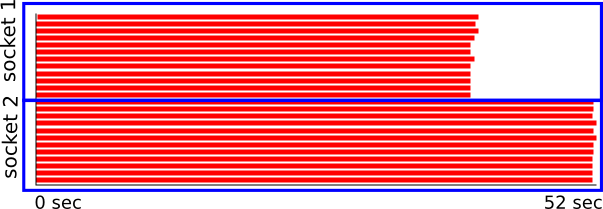
\includegraphics[width=\columnwidth]{power_aware_runtime/figures/swaptions-80watts-static}
        \caption{Static scheduling and 12 cores enabled.}
        \label{fig:swaptions_static_sched}
  \end{subfigure}
  \begin{subfigure}{\columnwidth}
        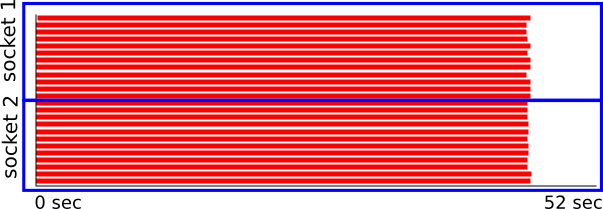
\includegraphics[width=\columnwidth]{power_aware_runtime/figures/swaptions-80watts-dynamic}
        \caption{Dynamic scheduling and 12 cores enabled.}
        \label{fig:swaptions_dynamic_sched}
  \end{subfigure}
  \caption{Executions of~\texttt{swaptions} 
                        under 40 W power capping.}
        \label{fig:load_balancing_sockets}
\vspace{.5cm}
\end{figure}



\subsection{Example with no Barrier or Synchronizations}
\label{sec:nobarriers}

\begin{figure}[ht]
  \begin{subfigure}{\columnwidth}
        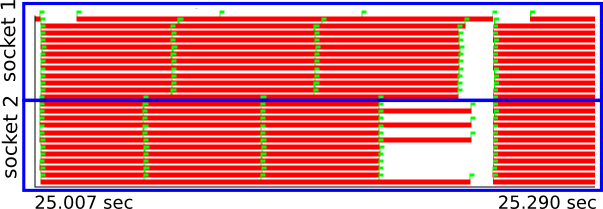
\includegraphics[width=\columnwidth]{power_aware_runtime/figures/blackscholes-80watts-even}
        \caption{Dynamic Scheduling and 12 cores enabled.}
        \label{fig:blackscholes_even_conf_trace}
  \end{subfigure}
  \begin{subfigure}{\columnwidth}
        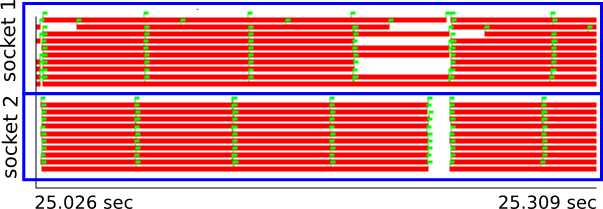
\includegraphics[width=\columnwidth]{power_aware_runtime/figures/blackscholes-80watts-best}
        \caption{Dynamic Scheduling and 10 cores enabled.}
        \label{fig:blackscholes_best_conf_trace}
  \end{subfigure}
  \caption{Executions of~\texttt{blackscholes} near a synchronization point under 40 W.}
  \label{fig:overprovisioning_sockets}%\
\vspace{.5cm}
\end{figure}


Figure~\ref{fig:load_balancing_sockets} compares two executions of the \texttt{swaptions}
benchmark~\cite{Chasapis:2015:PEI:2836331.2829952} on a NUMA node composed of two 12-core Intel Xeon E5-2695v2
sockets, each run with 24 threads and with power capped at 40W.  The x-axis of the figures
show time and the y-axis the activity of each of the 24 threads involved in the parallel
execution.  When the activity of a particular thread $i$ appears in red on time $t$, the
thread is doing useful work; if it appears in white, the thread is idling.  The scale of
the x-axis is the same in both figures and covers 0s to 52.8s.  In the run shown in
Figure~\ref{fig:swaptions_static_sched} the load is evenly distributed among all threads
statically using a naive distribution.  The reaction of the two sockets involved in the
parallel run is different, which makes the threads running on the faster socket (Threads
1-8) finish much earlier than the threads mapped to the slow socket (Threads 9-15). As a
result, threads from 1 to 8 are idle for 26\% of the execution time.

In Figure~\ref{fig:swaptions_dynamic_sched} we show a second parallel execution of the
same code, performed in the same NUMA node as above, but with dynamic scheduling.  For
this, we have over-decomposed the parallel execution into more tasks than cores and let
the parallel runtime system assign tasks to cores once they were idle.  In this way, the
cores on the fast socket executed some of the tasks that were assigned to cores on the
slower socket in the static case, which allows the whole parallel execution to achieve a
1.13x speedup over static scheduling.  This dynamic task assignment technique is
equivalent to the numerous work stealing approaches described in the
literature~\cite{Blumofe1999, Blumofe1995, Ravichandran2011, Zheng2011}: it is able to
deal with uneven hardware responses under restricted power budgets in the absence of
barriers or synchronization points.  Note however, that in order for conventional work
stealing to be effective, finer grain parallelism is prefered.  Introducing
synchronization and coarser parallel work unit limit the effectiveness of this method.


\subsection{Example with Barrier Operations}
\label{sec:barriers}

Figure~\ref{fig:overprovisioning_sockets} compares the behavior of two parallel executions
of the~\texttt{blackscholes} benchmark~\cite{Chasapis:2015:PEI:2836331.2829952} on the same NUMA node as the
one used above, again limited to 40W per socket.  In this case we show the behavior of the
parallel run around a barrier operation instead of the whole execution.  The x-axis
represents time and the y-axis shows the threads involved in the parallel execution.
Green flags mark the separation between the different pieces of sequential work in which
the parallel execution is split or, in other words, the tasks.

Figure~\ref{fig:blackscholes_even_conf_trace} shows the behavior of the dynamic task
scheduling using the same policy as above, with idle time shown in white.  While in the
absence of barriers this technique properly balances the load between the two 12-core
sockets, the results in this case clearly show that they fail in case of barriers: the
green flags show that the same tasks exhibit differences in execution time depending on
the socket they run on: around 74$\mu$s on average when run on the slow socket and 58 when
run on the fast one, despite each task executing the same computational workload.  Having
tasks with smaller granularity could offer more flexibility to the runtime's scheduler to 
better distribute the tasks among the sockets and cores, but it is not always possible to
decompose work into smaller units.  Furthermore, this requires alterations to the source
code of the application.  In this Chapter we propose a different approach to solve this
issue by redistributing power among sockets and finding the optimal concurrency level,
suitable for the specific socket and application.

Figure~\ref{fig:blackscholes_best_conf_trace} shows a second execution with the number of
threads per socket reduced to 10, i.e., 2 cores per socket or 4 cores total are left
unused during the execution.  In this example power is evenly distributed with 40W per
socket.  The average execution time of the tasks mapped to the slow socket gets reduced to
54$\mu$s, while the average time of those mapped to the fast socket takes 48$\mu$s to run.
This improved execution time is caused by the fact that the socket power budget is now
distributed among 10 cores instead of 12.  More importantly, the heterogeneous character
of the socket's response to the imposed power limit seems to be reduced by leaving 2 cores
idle.  This better balance between the two sockets significantly reduces the impact of
barriers and, therefore, their idle time.  Clearly, this is a much more balanced execution
than the one shown in Figure~\ref{fig:blackscholes_even_conf_trace}.  Overall, the
parallel run considering 10 cores per socket and dynamic task assignment shows a 1.21x
speedup with respect to the execution with 12 cores per socket combined with a dynamic
assignment.

This last example clearly shows that, under restricted power budgets and uneven hardware
reactions, operating with the maximum possible concurrency while dynamically balancing
load is insufficient since barrier points can introduce significant idling effects.  In
this cases, it can be better to restrict concurrency levels in order to homogenize the
hardware reaction to low power budgets.  Alternatively, it can also be helpful to unevenly
distribute the total power budget assigned to the multi-core sockets of a NUMA node in
order to compensate for varying processor efficiency, as we demonstrate in
Section~\ref{sec:static_analysis}.

\begin{figure}[ht]
        \centering
        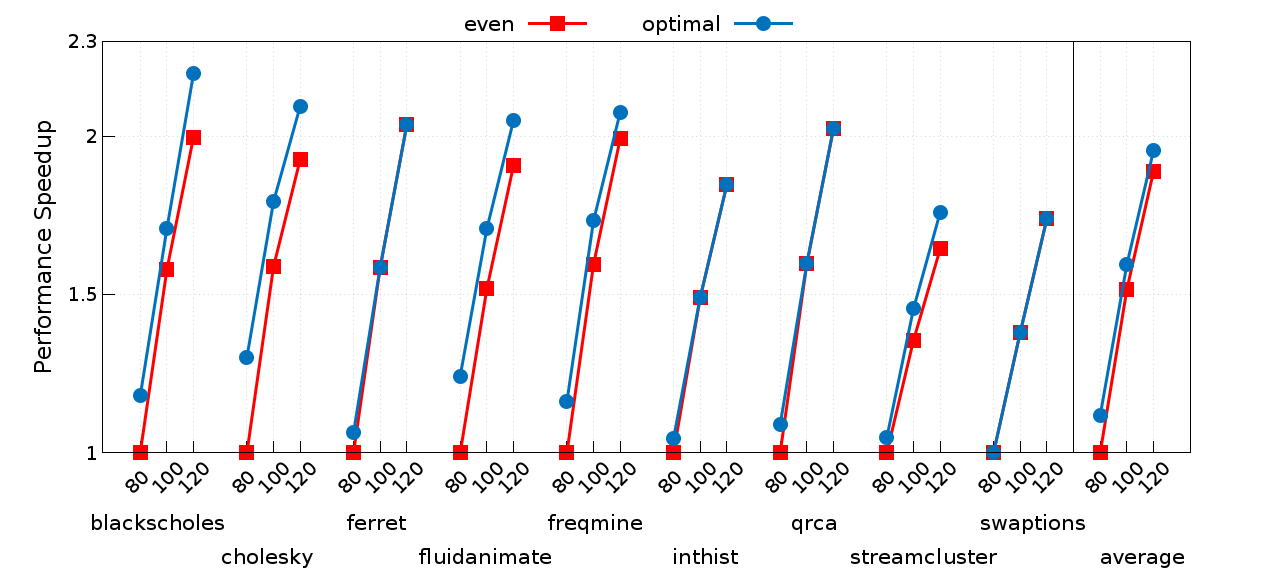
\includegraphics[width=\columnwidth]{./power_aware_runtime/figures/static_conf_analysis}
        \caption{Comparison between the even and the best configuration observed by application profiling. The speedup is computed over the execution of the even resource distribution for 80 W.}
        \label{fig:static_conf_analysis}
\vspace{.5cm}
\end{figure}


\begin{table}[]
\centering
\caption{Optimal configurations per application and power bound in terms or Watts and active cores per socket}
\label{table:optimal_configuration}
\def\arraystretch{1.5}%
\begin{tabular}{l|l|l|l|}
\cline{2-4}
                                    & 80 W & 100 W & 120 W \\ \hline
\multicolumn{1}{|l|}{\texttt{blackscholes}}  & 40-40 W, 10-10 cores & 55-45 W, 10-12 cores & 70-50 W, 12-10 cores \\ \hline
\multicolumn{1}{|l|}{\texttt{cholesky}}      & 30-50 W, 2-12 cores & 35-65 W, 2-12 cores & 30-90 W, 10-10 cores \\ \hline
\multicolumn{1}{|l|}{\texttt{ferret}}        & 40-40 W, 10-10 cores & 50-50 W, 12-12 cores & 60-60 W, 12-12 cores \\ \hline
\multicolumn{1}{|l|}{\texttt{fluidanimate}}  & 45-35 W, 10-6 cores & 55-45 W, 10-6 cores & 65-35 W, 10-6 cores \\ \hline
\multicolumn{1}{|l|}{\texttt{freqmine}}      & 45-35 W, 12-6 cores & 55-45 W, 10-12 cores & 65-55 W, 12-12 cores \\ \hline
\multicolumn{1}{|l|}{\texttt{inthist}}       & 40-40 W, 10-10 cores & 45-55 W, 12-12 cores & 60-60 W, 12-12 cores \\ \hline
\multicolumn{1}{|l|}{\texttt{qrca}}          & 45-35 W, 12-6 cores & 50-50 W, 12-12 cores & 60-60 W, 12-12 cores \\ \hline
\multicolumn{1}{|l|}{\texttt{streamcluster}} & 35-45 W, 2-12 cores & 60-40 W, 12-12 cores & 65-55 W, 12-12 cores \\ \hline
\multicolumn{1}{|l|}{\texttt{swaptions}}     & 40-40 W, 12-12 cores & 50-50 W, 12-12 cores & 60-60 W, 12-12 cores \\ \hline

\end{tabular}
\vspace{.5cm}
\end{table}


\section{Mitigating Heterogeneity}
\label{sec:static_analysis}
Following Sections~\ref{sec:nobarriers} and~\ref{sec:barriers}, which illustrate the
negative impact of heterogeneity introduced by power capping, we now provide a general
evaluation of the benefits of heterogeneity mitigation.  We consider a wide range of
parallel applications coming from many areas and we test their performance considering a
large range of power and concurrency configurations.  For each application and power
bound, we select the best configuration and compare its performance with the performance
obtained by deploying the naive even configuration --- assign half the power to each
thread and use all the available cores --- combined with traditional task scheduler and
balancer.


\subsection{Experimental Setup}
\label{sec:setup}
{\bf Applications:} we utilize nine OpenMP codes: six of them come from the PARSEC
benchmark suite~\cite{bienia2008, Chasapis:2015:PEI:2836331.2829952} (\texttt{black-scholes}, \texttt{ferret},
\texttt{fluidanimate}, \texttt{freqmine}, \texttt{streamcluster} and \texttt{swaptions}).
Two  of them are dense linear algebra routines (a cholesky matrix factorization,
\texttt{cholesky}, and a QR communication-avoiding code, \texttt{qrca}~\cite{Demmel1997})
and another one builds a histogram from a set of data points (\texttt{inthist}).  All of
these codes exploit task-based parallelism.  The benefits of using a programming model
which is coupled with a runtime system is that only the runtime needs to be modified to
accomodate our power budget and active core balancing algorithm, as well as the online
monitoring methodology.  Individual applications remain untouched, and the runtime handles
everything in a transparent manner.

{\bf Hardware and System Software:} NUMA nodes of the Catalyst
supercomputer~\cite{llnlconfluence} are composed of  two 12-core Intel Xeon E5-2695v2
sockets each. The applications run in top of the Nanos++ (v0.7a) parallel runtime
system~\cite{nanos}. We map one thread per active core.  To set power constraints and
measure power consumption on each socket, we use Intel's RAPL~\cite{IntelArcManual} .
These registers are accessed by our modified version of the Nanos++ runtime using the
libMSR library~\cite{libmsr}. 


{\bf Configurations:} We consider power bounds of 80W, 100W and 120W for total
node power.  This leaves 40W, 50W and 60W respectively per socket, which is 
between 35\% and 52\% of each socket's 115W TDP.
Although limiting socket power to 50\% or less may seem
aggressive, studies have shown that typical HPC workloads only use 60\%-85\% of
the available power on the socket \cite{Patki:2015:PRM:2749246.2749262}.  Moreover,
actual applications, such as the PARSECSs benchmarks, exhibit different
behavior at different execution stages.  As a result, an application may
reach its power peak for only a portion of its total execution.
Power limits above 50\% would have minimal impact on overall performance.
Furthermore,  there is a well established trend of an increase in manufacturing
variability in more modern processor models
\cite{Marathe:2017:ESP:3149412.3149421} and is expected to keep rising.  In
order for our study to be relevant for future processors, we choose a
configuration that creates enough variability between two sockets.  If we allow
a power limit of 80W, we consider 5 different ways of distributing the power
among the two sockets of the NUMA node: 30W:50W, 35W:45W, 40W:40W, 45W:35W and
50W:30W as well as 36 ways of specifying the maximum concurrency allowed in
each 2-socket NUMA node: 2-2, 4-2, 6-2, 8-2, 10-2, 12-2, 2-4, etc.  up to
12-12.  In total, this leads to a total of 180 combinations.  Similarly, when
allowing a power limit of 100W there are 8 ways of distributing it, which
combined with the 36 possible ways of distributing the concurrency, leads us to
a total of 324 combinations.  Similarly, when the total power budget reaches
120W, the total number of combinations is 468.  Overall, for each particular
application we have 972 different combinations.

{\bf Other Considerations:} The results of these experiments are machine dependent since
each particular 12-core socket reacts in a different way when a power limit is set.
Ideally, all  972 configurations per application should be executed on many NUMA nodes to
really account for many possible hardware reactions when a power limit is set.  However,
due to the size of our experimental campaign, we randomly chose a single 2-socket NUMA
node for each considered application and run all 972 combinations on it.  Although this
random choice can slightly influence the relative results between the benchmarks, the
general conclusions we extract from them remain unchanged.

\subsection{Evaluation}
\label{sec:static_evaluation}
In Figure~\ref{fig:static_conf_analysis} we show our experimental results.  On the x-axis
we represent all the considered applications and the three power bounds we consider: 80W,
100W and 120W.  In the y-axis we represent, for each particular application, the speedup
achieved over evenly distributing 80W among two sockets (40W per socket) and keeping 12
active cores per socket.  On average, the optimal configurations outperforms the totally
even distribution (50\% of the power and 12 cores per socket) by 11.8\% (80W), 7.3\%
(100W) and 7.6\% (120W).

Not surprisingly, the more restrictive the power capping is, the more beneficial the
optimal configuration becomes in terms of performance.  The uneven hardware reaction gets
exacerbated by restrictive power bounds, which gives more room for improvement when the
hardware is rebalanced by changing the power and concurrency assignation per socket.
Application-wise, the benefits are much larger for applications %with parallel schemes
composed of several execution phases separated by barriers, like \texttt{fluidanimate}
(24\% improvement) or \texttt{cholesky} (30\%).  On the other side, \texttt{swaptions}
does not get any benefit from our power rebalancing techniques since its lack of barriers
enables simple load balancing schemes to mitigate the hardware heterogeneous response, as
described in Section~\ref{sec:nobarriers}.

In Table~\ref{table:optimal_configuration} we list the optimal configuration for each
application and power bound.  As expected, for applications without barriers
(\texttt{swaptions} and \texttt{inthist}) the most balanced configurations (40W:40W and
12-12 active cores, 40W:40W and 10-10 cores respectively)  are optimal.  Since for these
applications the parallel runtime system successfully manages the load, there is no need
for system balancing by means of power or concurrency reassignment among the involved
threads.  On the other side, applications like \texttt{cholesky} or \texttt{fluidanimate}
do really benefit from leaving significant parts of the cores idle and rebalancing the
power accordingly.  Clearly, the hardware heterogeneity induced by setting a power bound
is not compensated by load balancing schemes delivered at the parallel runtime system side
and some concurrency and power rebalancing must be done to maximize the performance of
these applications.

This evaluation demonstrates that classical work stealing and load balancing techniques
are not able to compensate the heterogeneity induced by power capping, except for trivial
situations where a parallel code has no global barriers or synchronization points and the
size of the parallel work unit is small enough to allows versatile alternative scheduling
scenarios.  Since the potential benefits of power and concurrency rebalancing is up to
30\%, there is a need for developing techniques able to figure out the optimal
configuration within a single execution run. 


